\documentclass[modern]{aastex631}

% Affiliations
\newcommand{\cca}{Center for Computational Astrophysics, Flatiron Institute, 162 Fifth Avenue, New York, NY 10010, USA}
\newcommand{\sbu}{Department of Physics and Astronomy, Stony Brook University, Stony Brook, NY 11794, USA}
\newcommand{\pa}{Department of Physics and Astronomy, Northwestern University, 2145 Sheridan RD, Evanston, IL 60208, USA}
\newcommand{\ciera}{Center for Interdisciplinary Exploration and Research in Astrophysics (CIERA), Northwestern University, 1800 Sherman Ave, Evanston, IL 60201, USA}

% Editing commands
\newcommand{\todo}[1]{\textcolor{red}{TODO: #1}}

% Generated macros
\newcommand{\dNlogmpeak}{\ensuremath{100^{+44}_{-85}}}
\newcommand{\dNlogmpeakunits}{\ensuremath{\dNlogmpeak \, \mathrm{Gpc}^{-3} \, \mathrm{yr}^{-1}}}
\newcommand{\monepctplgplp}{\ensuremath{3.073^{+0.038}_{-0.053}}}
\newcommand{\monepctplgplpunits}{\ensuremath{\monepctplgplp \, M_\odot}}
\newcommand{\mpeakplgplp}{\ensuremath{9.18^{+0.96}_{-0.94}}}
\newcommand{\mpeakplgplpunits}{\ensuremath{\mpeakplgplp \, M_\odot}}
\newcommand{\alphatwoplgplp}{\ensuremath{-2.9^{+2.6}_{-1.7}}}
\newcommand{\mclow}{2.612}
\newcommand{\mclowunits}{\ensuremath{\mclow \, M_\odot}}\newcommand{\mchigh}{17.41}
\newcommand{\mchighunits}{\ensuremath{\mchigh \, M_\odot}}

\begin{document}
\title{Hiding Out at the Low End: Gaps and Peaks in the Black-Hole Mass Spectrum}

\author[0000-0003-1540-8562]{Will M. Farr}
\email{will.farr@stonybrook.edu}
\email{wfarr@flatironinstitute.org}
\affiliation{\sbu}
\affiliation{\cca}

\author[0000-0001-9236-5469]{Vassiliki Kalogera}
\email{vicky@northwestern.edu}
\affiliation{\pa}
\affiliation{\ciera}

\begin{abstract}
    It is not known whether there is a continum of masses of compact objects
    formed from stellar collapse from the heaviest neutron stars to the lightest
    black holes or whether there is a gap in the mass spectrum between these
    classes of objects.  The presence or absence of a mass gap has implications
    for the supernova mechanism, as well as being a fundamental property of the
    compact object mass function.  In X-ray binaries containing black holes a
    gap is observed, but it is not known whether this is representative of a
    true gap in the mass function or due to selection effects or systematic
    biases in mass estimation.  A small number of black holes have been observed
    with luminous companions in non-interacting orbits, but as yet the sample is
    too small to assess the existence of a gap, and in any case selection
    effects in this sample are hard to quantify \todo{Check this!}.  Binary
    black hole mergers detected from gravitational waves in the GWTC-3 transient
    catalog furnish a large sample of several tens of low-mass black holes with
    a well-understood selection function.  Here we analyze the 15 GWTC-3 merger
    events with black hole masses in $3 \, M_\odot < m_2 < m_1 < 20 \, M_\odot$
    in detail to uncover the structure of the low-mass black hole mass function
    in these systems.  Using several flexible parameterized models for the mass
    function, we find a sharp peak (width $\lesssim 20\%$) in the mass function
    at $m = 9.47^{+0.52}_{-0.58} \, M_\odot$, associated with merger rates $m_1
    m_2 \mathrm{d} N / \mathrm{d} m_1 \mathrm{d} m_2 \mathrm{d} V \mathrm{d} t =
    270^{+270}_{-150} \, \mathrm{Gpc}^{-3} \, \mathrm{yr}^{-1}$.  The mass
    function falls by at least an order of magnitude both below and above this
    peak.  Toward the lowest masses, the mass function may or may not flatten;
    we find that the $1\%$ black hole mass in our most flexible model is
    $m_{1\%} = 3.28^{+1.19}_{-0.13} \, M_\odot$. In other words, this sample of
    low-mass black holes does not require a mass gap but may permit one;
    observations in the currently-ongoing ``O4'' observation run should
    distinguish these possibilities.  Toward higher masses, the mass function
    declines to our upper limit $m = 20 \, M_\odot$ steeply, with power law
    slopes $\mathrm{d} N / \mathrm{d} m \sim m^{-\alpha}$, $\alpha =
    -4.9^{+3.1}_{-3.3}$.  The presence of a peak at $m \sim 9 \, M_\odot$ is
    suggested by several models of stellar evolution.
\end{abstract}

\section{Introduction}

\begin{figure}
    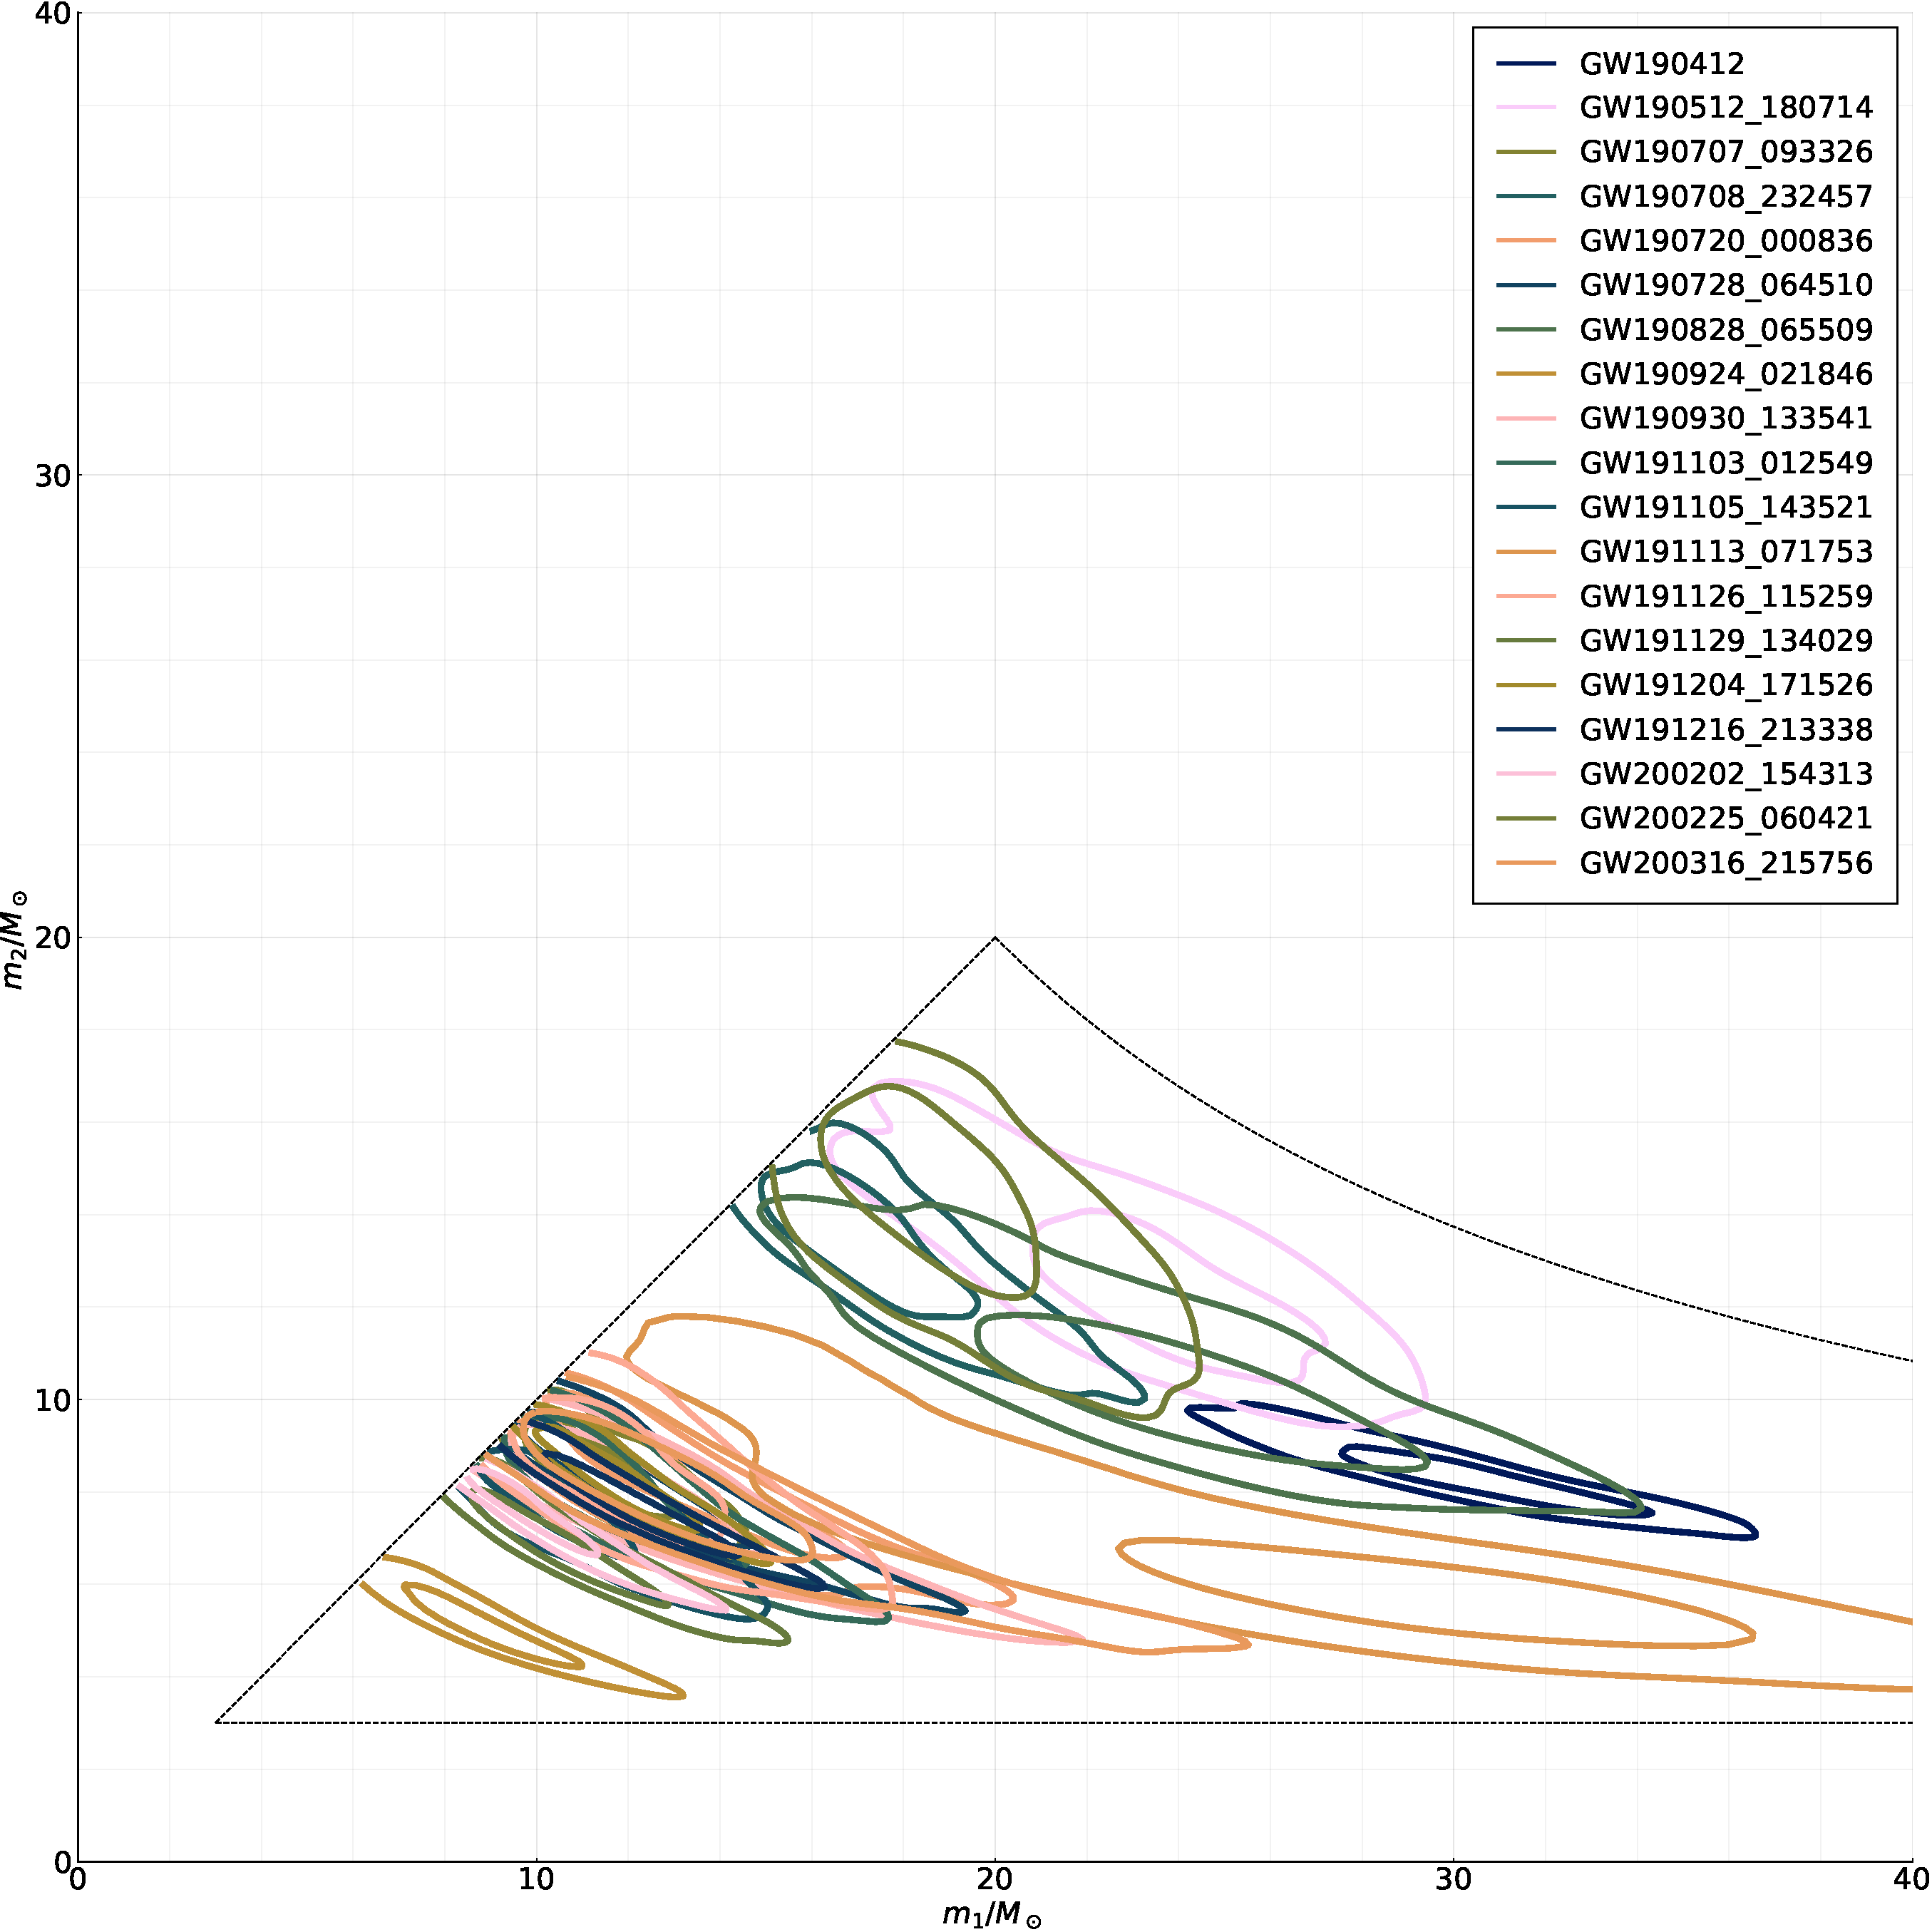
\includegraphics[width=\columnwidth]{figures/m1-m2-contour.pdf}
    \caption{\label{fig:m1-m2-contour} Contour plot of the likelihood functions
    for the primary and secondary black hole masses in the events considered in
    this analysis.  The contours show credible regions containing $50\%$ and
    $90\%$ of the likelihood for each event.  The dashed lines show our
    selection cuts, with $m_2 > 3 \, M_\odot$ and $\mclowunits < M_c <
    \mchighunits$.}
\end{figure}

\begin{figure}
    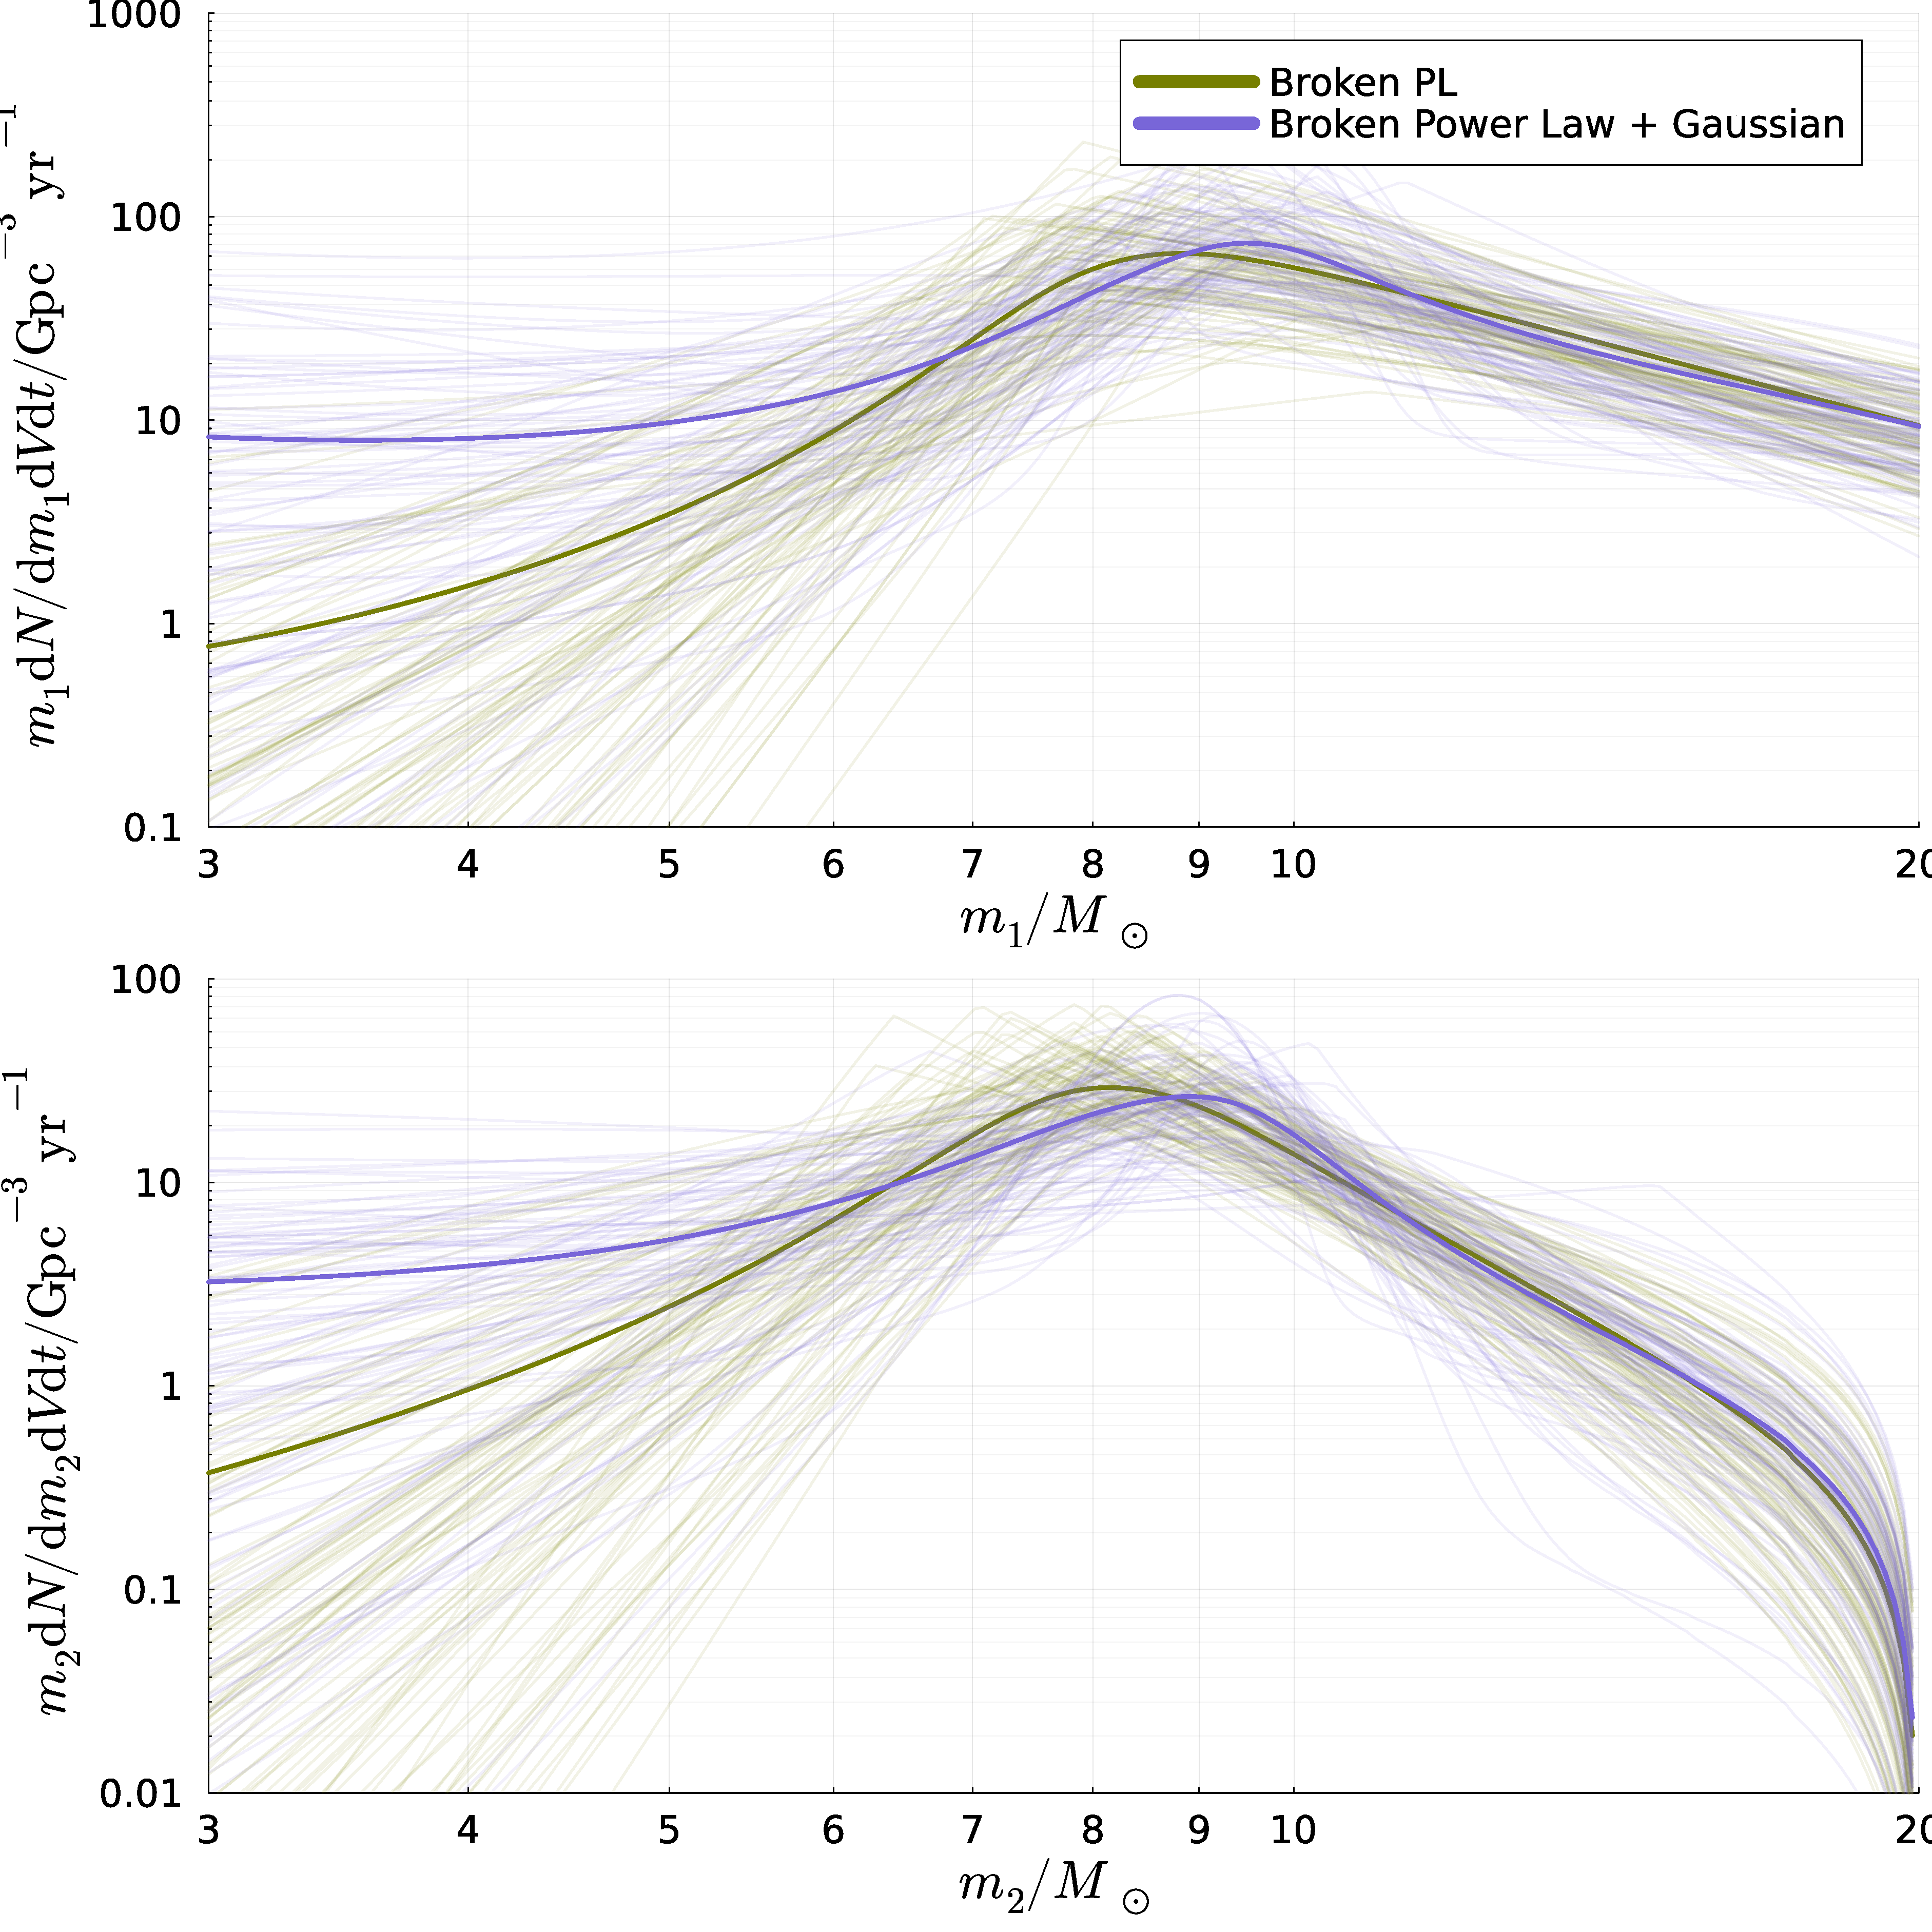
\includegraphics[width=\columnwidth]{figures/dNdm_traces.pdf}
    \caption{\label{fig:dNdm-traces} Inferred mass functions for $3 \, M_\odot <
    m_2 < m_1 < 20 \, M_\odot$ from two models; both primary and secodary
    (marginal) mass functions are shown.  Dark lines show the posterior mean
    mass function; light lines are individual draws from the posterior over mass
    functions.}
\end{figure}

\end{document}
